%----------------------------------------------------------------------------------------
%	PACKAGES AND OTHER DOCUMENT CONFIGURATIONS
%----------------------------------------------------------------------------------------

\documentclass{article}

\usepackage{fancyhdr} % Required for custom headers
\usepackage{lastpage} % Required to determine the last page for the footer
\usepackage{extramarks} % Required for headers and footers
\usepackage[usenames,dvipsnames]{color} % Required for custom colors
\usepackage{graphicx} % Required to insert images
\usepackage{listings} % Required for insertion of code
\usepackage{courier} % Required for the courier font
\usepackage{lipsum} % Used for inserting dummy 'Lorem ipsum' text into the template
\usepackage{epstopdf}
\usepackage{fancyhdr}
\usepackage{combelow}
\usepackage{enumerate}
\usepackage{amssymb,amsmath}
\usepackage{moreverb}
\usepackage{listings}
\usepackage{multirow}
\usepackage{verbatim}
\usepackage{epsfig}
\usepackage{epstopdf}
\usepackage{tabularx}
\usepackage{color}
\usepackage{subcaption}
\usepackage{tabulary}
\usepackage{wrapfig}
\usepackage{hyperref}
\usepackage[utf8x]{inputenc}

% Margins
\topmargin=-0.45in
\evensidemargin=0in
\oddsidemargin=0in
\textwidth=6.5in
\textheight=9.0in
\headsep=0.25in
\headheight=33pt

\linespread{1} % Line spacing

% Set up the header and footer
\pagestyle{fancyplain}
\fancyhf{}
\lhead{\MNTitle} % Top left header
%\chead{\MNTitleShort} % Top center head
\rhead{
\includegraphics[width=2cm]{Logo.jpg}} % Top right header
\lfoot{\MNClass} % Bottom left footer
\cfoot{} % Bottom center footer
\rfoot{Pagina\ \thepage\ din\ \protect\pageref{LastPage}} % Bottom right footer
\renewcommand\headrulewidth{0.4pt} % Size of the header rule
\renewcommand\footrulewidth{0.4pt} % Size of the footer rule

%----------------------------------------------------------------------------------------
%	CODE INCLUSION CONFIGURATION
%----------------------------------------------------------------------------------------

\definecolor{mygreen}{rgb}{0,0.6,0}
\definecolor{mygray}{rgb}{0.5,0.5,0.5}
\definecolor{mymauve}{rgb}{0.58,0,0.82}

\lstset{ %
  backgroundcolor=\color{white},		% choose the background color; you must add \usepackage{color} or \usepackage{xcolor}
  basicstyle=\small\ttfamily,		% the size of the fonts that are used for the code
  breakatwhitespace=false,			% sets if automatic breaks should only happen at whitespace
  breaklines=true,					% sets automatic line breaking
  captionpos=b,						% sets the caption-position to bottom
  commentstyle=\color{mygreen},		% comment style
  deletekeywords={...},				% if you want to delete keywords from the given language
  escapeinside={\%*}{*)},			% if you want to add LaTeX within your code
  extendedchars=true,				% lets you use non-ASCII characters; for 8-bits encodings only, does not work with UTF-8
  frame=single,						% adds a frame around the code
  keepspaces=true,					% keeps spaces in text, useful for keeping indentation of code (possibly needs columns=flexible)
  keywordstyle=\color{black},			% keyword style
  language=Octave,					% the language of the code
  morekeywords={*,...},				% if you want to add more keywords to the set
  numbers=left,						% where to put the line-numbers; possible values are (none, left, right)
  numbersep=6pt,						% how far the line-numbers are from the code
  numberstyle=\tiny\color{mygray},	% the style that is used for the line-numbers
  rulecolor=\color{black},			% if not set, the frame-color may be changed on line-breaks within not-black text (e.g. comments (green here))
  showspaces=false,					% show spaces everywhere adding particular underscores; it overrides 'showstringspaces'
  showstringspaces=false,			% underline spaces within strings only
  showtabs=false,					% show tabs within strings adding particular underscores
  stepnumber=1,						% the step between two line-numbers. If it's 1, each line will be numbered
  stringstyle=\color{mymauve},		% string literal style
  tabsize=2,							% sets default tabsize to 2 spaces
  title=\lstname						% show the filename of files included with \lstinputlisting; also try caption instead of title
}

% Creates a new command to include a perl script, the first parameter is the filename of the script (without .pl), the second parameter is the caption
\newcommand{\octavescript}[2]{
\begin{itemize}
\item[]\lstinputlisting[caption=#2,label=#1]{#1.m}
\end{itemize}
}

%----------------------------------------------------------------------------------------
%	DOCUMENT STRUCTURE COMMANDS
%	Skip this unless you know what you're doing
%----------------------------------------------------------------------------------------

\setcounter{secnumdepth}{0} % Removes default section numbers
\newcounter{ProblemCounter} % Creates a counter to keep track of the number of problems

\newcommand{\ProblemName}{}
\newenvironment{Problem}[1][Sectiunea \arabic{ProblemCounter}]{ % Makes a new environment called Problem which takes 1 argument (custom name) but the default is "Problem #"
\stepcounter{ProblemCounter} % Increase counter for number of problems
\renewcommand{\ProblemName}{#1} % Assign \ProblemName the name of the problem
\section{\ProblemName} % Make a section in the document with the custom problem count
}{}

\newcommand{\ProblemAnswer}[1]{ % Defines the problem answer command with the content as the only argument
\noindent\framebox[\columnwidth][c]{\begin{minipage}{0.98\columnwidth}#1\end{minipage}} % Makes the box around the problem answer and puts the content inside
}

\newcommand{\SectionName}{}
\newenvironment{Section}[1]{ % New environment for sections within  problems, takes 1 argument - the name of the section
\renewcommand{\SectionName}{#1} % Assign \SectionName to the name of the section from the environment argument
\subsection{\SectionName} % Make a subsection with the custom name of the subsection
}{}

%----------------------------------------------------------------------------------------
%	NAME AND CLASS SECTION
%----------------------------------------------------------------------------------------

\newcommand{\MNTitleShort}{Tema\ \#3} % Assignment title
\newcommand{\MNTitle}{Tema\ \#3 Site web utilizare resurse IA} % Assignment title
\newcommand{\MNDueDate}{Ultimul laborator} % Due date
\newcommand{\MNClass}{SISTEME TOLERANTE LA DEFECTE} % Course/class
\newcommand{\MNClassTime}{} % Class/lecture time
\newcommand{\MNClassInstructor}{Cristian Chilipirea} % Teacher/lecturer
\newcommand{\MNAuthorName}{Cristian Chilipirea} % Your name

%----------------------------------------------------------------------------------------
%	TITLE PAGE
%----------------------------------------------------------------------------------------

\title{
%\vspace{2in}
\textmd{\textbf{\MNClass \\ \MNTitle}}\\
\normalsize\vspace{0.1in}\small{Termen de predare: \MNDueDate}\\
}

\date{} % Insert date here if you want it to appear below your name

%----------------------------------------------------------------------------------------

\begin{document}

\maketitle

%----------------------------------------------------------------------------------------
%    TABLE OF CONTENTS
%----------------------------------------------------------------------------------------

%\setcounter{tocdepth}{1} % Uncomment this line if you don't want subsections listed in the ToC

%\newpage
%\tableofcontents
%\newpage


%----------------------------------------------------------------------------------------
%    OBIECTIVELE TEMEI DE CASA
%----------------------------------------------------------------------------------------
\section{Obiective}

Scopul acestei teme este de a implementa, folosindu-vă de tehnologii serverless un site web care să faciliteze folosirea unei tehnologii de IA pusă la dispoziție prin Azure.

%----------------------------------------------------------------------------------------
%    PROBLEM 1
%----------------------------------------------------------------------------------------

% To have just one problem per page, simply put a \clearpage after each problem

\begin{Problem}[Enunț]

Această temă este personalizată pentru \textbf{NUMESTUDENT}.

Obiectivul temei este de a crea un website ce va permite upload-ul unui fișier care va fi procesat apoi de un sistem de IA. Site-ul va reține un istoric cu toate cererile făcute acestuia.

Arhitectura site-ului va conține următoarele componente \textbf{Serverless}:

1. Un web service ce va conține un site web. În site-ul web va exista un formular de upload fișiere. O dată uploadat fișierul va fi procesat/stocat folosind alte servicii. Sub formularul de upload va exista o listă reprezentând un istoric cu toate fișierele uploadate pe site, link-uri către acestea, data și ora upload-ului și rezultatele procesării acestora cu tehnica IA cerută.

2. Fișierele vor fi stocate în blob storage.

3. Informațiile despre fișiere (nume, adresa, timestamp, rezultat procesare) vor fi stocate într-o bază de date SQL.

4. Fișierele vor fi procesate folosind un serviciu de IA (speech-to-text, translate, speech translation, face detection, form recognizer, OCR, image tagging, image description, sentiment analysis, entity extraction, anomaly detection, brand detection). Acestei teme îi este asignat serviciul \textbf{IAOPTION}.

\begin{figure}[th]
\centering
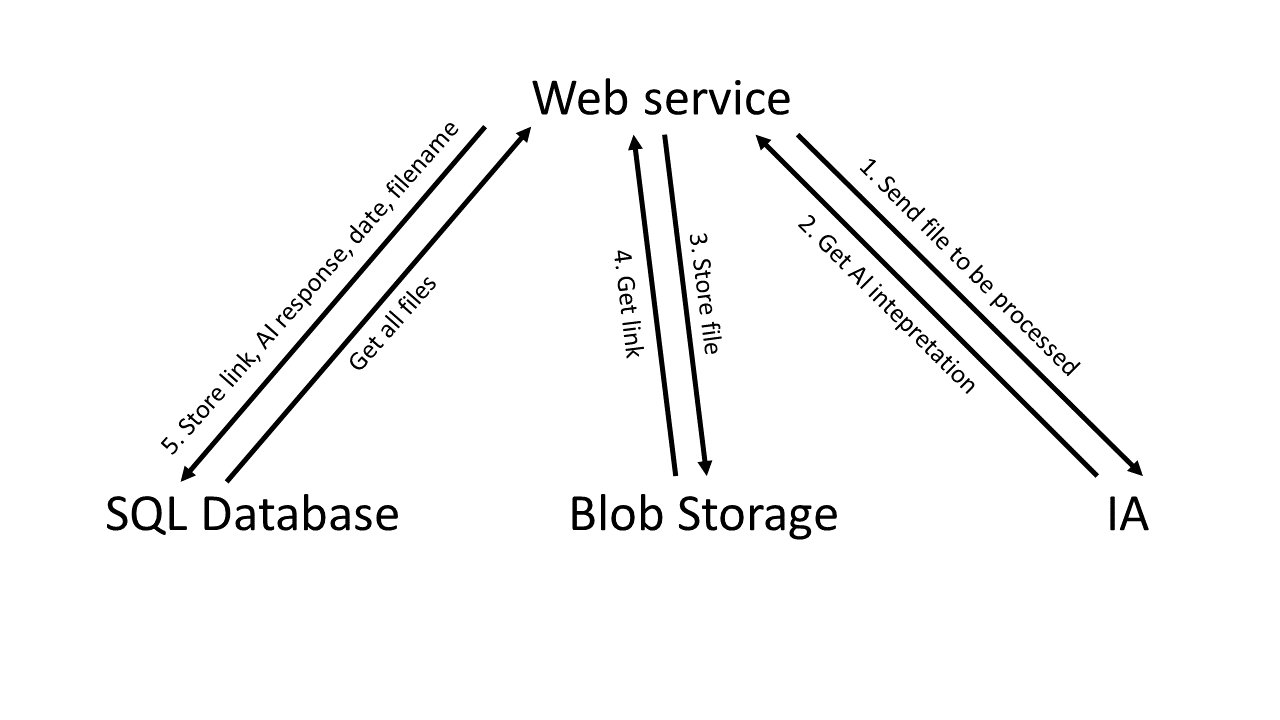
\includegraphics[width=11cm]{architecture.png}
  \caption{Exemplu de arhitectura}
  \label{fig:architecture_diagram}
\end{figure}

Figura~\ref{fig:architecture_diagram} prezintă o arhitectura generică pentru site-ul web cerut.

Website-ul poate fi creat în PHP sau în alt limbaj cerut. Cei care au cerut pentru tema 2 alte limbaje au opțiunea între PHP și acele limbaje. În cazul alegerii altui limbaj este obligatorie anunțarea în prima săptămână după primirea temei.

Fiecare sistem de IA are specificații un pic diferite. A se vedea mai jos:
\begin{itemize}
    \item speech-to-text - input fișier audio - output text cu ce se aude
    \item translate - input fișier text - output text tradus - va conține selector de limbă în site
    \item face detection - input poză cu o față - output poziția feței în imagine
    \item form recognizer - input poză cu un formular, un tabel - output text care descrie ce e în poză
    \item OCR - input poză cu text în imagine - output textul
    \item image tagging - input poză cu mai multe obiecte - output listă cu acele obiecte
    \item image description - input poză cu mai multe obiecte - output o descriere a pozei
    \item sentiment analysis - input fișier text - output listă de sentimente cu procente
    \item entity extraction - input fișier text - output listă de elemente importante din fișier
    \item anomaly detection - input fișier csv cu date - output momentele în care apar anomalii în acele date
    \item brand detection - input poză cu un produs al unei companii cu logo-ul companiei - output numele companiei
\end{itemize}

\end{Problem}

\begin{Problem}[Prezentare și punctare]

În ziua prezentării, întreaga infrastructură trebuie să fie în picioare și funcțională. Se va indica link-ul către site-ul web.

Se va pregăti o arhivă .zip ce conține un fișier README ce indică pașii efectuați pentru construcția sistemului și orice cod necesar implementării. Această arhivă va fi verificată pentru plagiat.

    Distribuția punctajului este următoarea:
\begin{itemize}
    \item 70 puncte - Site-ul funcționează conform specificațiilor
    \item 30 puncte - Demonstrați că ați testat extensiv site-ul creat identificând cazuri în care sistemul IA nu funcționează după așteptări și cazuri când funcționează surprinzător de bine (gen merge pe imagini blurry sau audio cu mult zgomot)

\end{itemize}

\end{Problem}

\end{document}